\documentclass[12pt,twoside]{article}
\newcommand{\reporttitle}{ElasticFusion on the Google Tango Tablet}
\newcommand{\reportauthor}{Jiahao Lin}
\newcommand{\reporttype}{Final Project Report}
\newcommand{\cid}{00837321}
\newcommand{\supervisor}{Dr Stefan Leutenegger}

% include files that load packages and define macros
%%%%%%%%%%%%%%%%%%%%%%%%%%%%%%%%%%%%%%%%%
% University Assignment Title Page 
% LaTeX Template
% Version 1.0 (27/12/12)
%
% This template has been downloaded from:
% http://www.LaTeXTemplates.com
%
% Original author:
% WikiBooks (http://en.wikibooks.org/wiki/LaTeX/Title_Creation)
%
% License:
% CC BY-NC-SA 3.0 (http://creativecommons.org/licenses/by-nc-sa/3.0/)
% 
% Instructions for using this template:
% This title page is capable of being compiled as is. This is not useful for 
% including it in another document. To do this, you have two options: 
%
% 1) Copy/paste everything between \begin{document} and \end{document} 
% starting at \begin{titlepage} and paste this into another LaTeX file where you 
% want your title page.
% OR
% 2) Remove everything outside the \begin{titlepage} and \end{titlepage} and 
% move this file to the same directory as the LaTeX file you wish to add it to. 
% Then add \input{./title_page_1.tex} to your LaTeX file where you want your
% title page.
%
%----------------------------------------------------------------------------------------
%	PACKAGES AND OTHER DOCUMENT CONFIGURATIONS
%----------------------------------------------------------------------------------------
\usepackage{ifxetex}
\usepackage{textpos}
\usepackage{natbib}
\usepackage{kpfonts}
\usepackage[a4paper,hmargin=2.8cm,vmargin=2.0cm,includeheadfoot]{geometry}
\usepackage{ifxetex}
\usepackage{stackengine}
\usepackage{tabularx,longtable,multirow,subfigure,caption}%hangcaption
\usepackage{fncylab} %formatting of labels
\usepackage{fancyhdr}
\usepackage{color}
\usepackage[tight,ugly]{units}
\usepackage{url}
\usepackage{float}
\usepackage[english]{babel}
\usepackage{amsmath}
\usepackage{graphicx}
\usepackage[colorinlistoftodos]{todonotes}
\usepackage{dsfont}
\usepackage{epstopdf} % automatically replace .eps with .pdf in graphics
\usepackage{natbib}
\usepackage{backref}
\usepackage{array}
\usepackage{latexsym}
\usepackage{etoolbox}

\usepackage{enumerate} % for numbering with [a)] format 



\ifxetex
\usepackage{fontspec}
\setmainfont[Scale=.8]{OpenDyslexic-Regular}
\else
\usepackage[pdftex,pagebackref,hypertexnames=false,colorlinks]{hyperref} % provide links in pdf
\hypersetup{pdftitle={},
  pdfsubject={}, 
  pdfauthor={\reportauthor},
  pdfkeywords={}, 
  pdfstartview=FitH,
  pdfpagemode={UseOutlines},% None, FullScreen, UseOutlines
  bookmarksnumbered=true, bookmarksopen=true, colorlinks,
    citecolor=black,%
    filecolor=black,%
    linkcolor=black,%
    urlcolor=black}
\usepackage[all]{hypcap}
\fi

\usepackage{tcolorbox}

% various theorems
\usepackage{ntheorem}
\theoremstyle{break}
\newtheorem{lemma}{Lemma}
\newtheorem{theorem}{Theorem}
\newtheorem{remark}{Remark}
\newtheorem{definition}{Definition}
\newtheorem{proof}{Proof}

% example-environment
\newenvironment{example}[1][]
{ 
\vspace{4mm}
\noindent\makebox[\linewidth]{\rule{\hsize}{1.5pt}}
\textbf{Example #1}\\
}
{ 
\noindent\newline\makebox[\linewidth]{\rule{\hsize}{1.0pt}}
}



%\renewcommand{\rmdefault}{pplx} % Palatino
% \renewcommand{\rmdefault}{put} % Utopia

\ifxetex
\else
\renewcommand*{\rmdefault}{bch} % Charter
\renewcommand*{\ttdefault}{cmtt} % Computer Modern Typewriter
%\renewcommand*{\rmdefault}{phv} % Helvetica
%\renewcommand*{\rmdefault}{iwona} % Avant Garde
\fi

\setlength{\parindent}{0em}  % indentation of paragraph

\setlength{\headheight}{14.5pt}
\pagestyle{fancy}
\fancyfoot[ER,OL]{\thepage}%Page no. in the left on
                                %odd pages and on right on even pages
\fancyfoot[OC,EC]{\sffamily }
\renewcommand{\headrulewidth}{0.1pt}
\renewcommand{\footrulewidth}{0.1pt}
\captionsetup{margin=10pt,font=small,labelfont=bf}


%--- chapter heading

\def\@makechapterhead#1{%
  \vspace*{10\p@}%
  {\parindent \z@ \raggedright %\sffamily
        %{\Large \MakeUppercase{\@chapapp} \space \thechapter}
        %\\
        %\hrulefill
        %\par\nobreak
        %\vskip 10\p@
    \interlinepenalty\@M
    \Huge \bfseries 
    \thechapter \space\space #1\par\nobreak
    \vskip 30\p@
  }}

%---chapter heading for \chapter*  
\def\@makeschapterhead#1{%
  \vspace*{10\p@}%
  {\parindent \z@ \raggedright
    \sffamily
    \interlinepenalty\@M
    \Huge \bfseries  
    #1\par\nobreak
    \vskip 30\p@
  }}
  



% %%%%%%%%%%%%% boxit
\def\Beginboxit
   {\par
    \vbox\bgroup
	   \hrule
	   \hbox\bgroup
		  \vrule \kern1.2pt %
		  \vbox\bgroup\kern1.2pt
   }

\def\Endboxit{%
			      \kern1.2pt
		       \egroup
		  \kern1.2pt\vrule
		\egroup
	   \hrule
	 \egroup
   }	

\newenvironment{boxit}{\Beginboxit}{\Endboxit}
\newenvironment{boxit*}{\Beginboxit\hbox to\hsize{}}{\Endboxit}



\allowdisplaybreaks

\makeatletter
\newcounter{elimination@steps}
\newcolumntype{R}[1]{>{\raggedleft\arraybackslash$}p{#1}<{$}}
\def\elimination@num@rights{}
\def\elimination@num@variables{}
\def\elimination@col@width{}
\newenvironment{elimination}[4][0]
{
    \setcounter{elimination@steps}{0}
    \def\elimination@num@rights{#1}
    \def\elimination@num@variables{#2}
    \def\elimination@col@width{#3}
    \renewcommand{\arraystretch}{#4}
    \start@align\@ne\st@rredtrue\m@ne
}
{
    \endalign
    \ignorespacesafterend
}
\newcommand{\eliminationstep}[2]
{
    \ifnum\value{elimination@steps}>0\leadsto\quad\fi
    \left[
        \ifnum\elimination@num@rights>0
            \begin{array}
            {@{}*{\elimination@num@variables}{R{\elimination@col@width}}
            |@{}*{\elimination@num@rights}{R{\elimination@col@width}}}
        \else
            \begin{array}
            {@{}*{\elimination@num@variables}{R{\elimination@col@width}}}
        \fi
            #1
        \end{array}
    \right]
    & 
    \begin{array}{l}
        #2
    \end{array}
    &%                                    moved second & here
    \addtocounter{elimination@steps}{1}
}
\makeatother

%% Fast macro for column vectors
\makeatletter  
\def\colvec#1{\expandafter\colvec@i#1,,,,,,,,,\@nil}
\def\colvec@i#1,#2,#3,#4,#5,#6,#7,#8,#9\@nil{% 
  \ifx$#2$ \begin{bmatrix}#1\end{bmatrix} \else
    \ifx$#3$ \begin{bmatrix}#1\\#2\end{bmatrix} \else
      \ifx$#4$ \begin{bmatrix}#1\\#2\\#3\end{bmatrix}\else
        \ifx$#5$ \begin{bmatrix}#1\\#2\\#3\\#4\end{bmatrix}\else
          \ifx$#6$ \begin{bmatrix}#1\\#2\\#3\\#4\\#5\end{bmatrix}\else
            \ifx$#7$ \begin{bmatrix}#1\\#2\\#3\\#4\\#5\\#6\end{bmatrix}\else
              \ifx$#8$ \begin{bmatrix}#1\\#2\\#3\\#4\\#5\\#6\\#7\end{bmatrix}\else
                 \PackageError{Column Vector}{The vector you tried to write is too big, use bmatrix instead}{Try using the bmatrix environment}
              \fi
            \fi
          \fi
        \fi
      \fi
    \fi
  \fi 
}  
\makeatother

\robustify{\colvec}

%%% Local Variables: 
%%% mode: latex
%%% TeX-master: "notes"
%%% End: 
 % various packages needed for maths etc.
% quick way of adding a figure
\newcommand{\fig}[3]{
 \begin{center}
 \scalebox{#3}{\includegraphics[#2]{#1}}
 \end{center}
}

%\newcommand*{\point}[1]{\vec{\mkern0mu#1}}
\newcommand{\ci}[0]{\perp\!\!\!\!\!\perp} % conditional independence
\newcommand{\point}[1]{{#1}} % points 
\renewcommand{\vec}[1]{{\boldsymbol{{#1}}}} % vector
\newcommand{\mat}[1]{{\boldsymbol{{#1}}}} % matrix
\newcommand{\R}[0]{\mathds{R}} % real numbers
\newcommand{\Z}[0]{\mathds{Z}} % integers
\newcommand{\N}[0]{\mathds{N}} % natural numbers
\newcommand{\nat}[0]{\mathds{N}} % natural numbers
\newcommand{\Q}[0]{\mathds{Q}} % rational numbers
\ifxetex
\newcommand{\C}[0]{\mathds{C}} % complex numbers
\else
\newcommand{\C}[0]{\mathds{C}} % complex numbers
\fi
\newcommand{\tr}[0]{\text{tr}} % trace
\renewcommand{\d}[0]{\mathrm{d}} % total derivative
\newcommand{\inv}{^{-1}} % inverse
\newcommand{\id}{\mathrm{id}} % identity mapping
\renewcommand{\dim}{\mathrm{dim}} % dimension
\newcommand{\rank}[0]{\mathrm{rk}} % rank
\newcommand{\determ}[1]{\mathrm{det}(#1)} % determinant
\newcommand{\scp}[2]{\langle #1 , #2 \rangle}
\newcommand{\kernel}[0]{\mathrm{ker}} % kernel/nullspace
\newcommand{\img}[0]{\mathrm{Im}} % image
\newcommand{\idx}[1]{{(#1)}}
\DeclareMathOperator*{\diag}{diag}
\newcommand{\E}{\mathds{E}} % expectation
\newcommand{\var}{\mathds{V}} % variance
\newcommand{\gauss}[2]{\mathcal{N}\big(#1,\,#2\big)} % gaussian distribution N(.,.)
\newcommand{\gaussx}[3]{\mathcal{N}\big(#1\,|\,#2,\,#3\big)} % gaussian distribution N(.|.,.)
\newcommand{\gaussBig}[2]{\mathcal{N}\left(#1,\,#2\right)} % see above, but with brackets that adjust to the height of the arguments
\newcommand{\gaussxBig}[3]{\mathcal{N}\left(#1\,|\,#2,\,#3\right)} % see above, but with brackets that adjust to the height of the arguments
\DeclareMathOperator{\cov}{Cov} % covariance (matrix) 
\ifxetex
\renewcommand{\T}[0]{^\top} % transpose
\else
\newcommand{\T}[0]{^\top}
\fi
% matrix determinant
\newcommand{\matdet}[1]{
\left|
\begin{matrix}
#1
\end{matrix}
\right|
}



%%% various color definitions
\definecolor{darkgreen}{rgb}{0,0.6,0}

\newcommand{\blue}[1]{{\color{blue}#1}}
\newcommand{\red}[1]{{\color{red}#1}}
\newcommand{\green}[1]{{\color{darkgreen}#1}}
\newcommand{\orange}[1]{{\color{orange}#1}}
\newcommand{\magenta}[1]{{\color{magenta}#1}}
\newcommand{\cyan}[1]{{\color{cyan}#1}}


% redefine emph
\renewcommand{\emph}[1]{\blue{\bf{#1}}}

% place a colored box around a character
\gdef\colchar#1#2{%
  \tikz[baseline]{%
  \node[anchor=base,inner sep=2pt,outer sep=0pt,fill = #2!20] {#1};
    }%
}%
 % short-hand notation and macros


%%%%%%%%%%%%%%%%%%%%%%%%%%%%

\begin{document}

% front page
% Last modification: 2016-09-29 (Marc Deisenroth)
\begin{titlepage}

\newcommand{\HRule}{\rule{\linewidth}{0.5mm}} % Defines a new command for the horizontal lines, change thickness here


%----------------------------------------------------------------------------------------
%	LOGO SECTION
%----------------------------------------------------------------------------------------


\includegraphics[width = 4cm]{./figures/imperial}\\[0.5cm]

\begin{center} % Center remainder of the page

%----------------------------------------------------------------------------------------
%	HEADING SECTIONS
%----------------------------------------------------------------------------------------
\textsc{\LARGE \reporttype}\\[1.5cm]
\textsc{\Large Imperial College London}\\[0.5cm]
\textsc{\large Department of Computing}\\[0.5cm]
%----------------------------------------------------------------------------------------
%	TITLE SECTION
%----------------------------------------------------------------------------------------

\HRule \\[0.4cm]
{ \huge \bfseries \reporttitle}\\ % Title of your document
\HRule \\[1.5cm]
\end{center}
%----------------------------------------------------------------------------------------
%	AUTHOR SECTION
%----------------------------------------------------------------------------------------

%\begin{minipage}{0.4\hsize}
\begin{flushleft} \large
\textit{Author:}\\
\reportauthor~(CID: \cid) % Your name
\\Supervisor: \supervisor\\
\end{flushleft}
\vspace{2cm}
\makeatletter
Date: \@date

\vfill % Fill the rest of the page with whitespace



\makeatother


\end{titlepage}


%%%%%%%%%%%%%%%%%%%%%%%%%%%% Main document

\section{Abstract}
Abstract\\
The abstract is a very brief summary of the report's contents. It should be about half a page long. Somebody unfamiliar with your project should have a good idea of what it's about having read the abstract alone and will know whether it will be of interest to them. Note that the abstract is a summary of the entire project including its conclusions. A common mistake is to provide only introductory elements in the abstract without saying what has been achieved.\\

=============\\

In recent years, Google has released an augmented reality Computing platform, Tango\footnote{\url{https://get.google.com/tango/}}. Supporting by with this platform, Google's Tango tablet is an Android device that equip with sensors that enable computer vision functionalities, Including NVIDIA Tegra K1 processor, 4MP color camera, fisheye-lens (motion-tracking) camera, Inertial Measurement Unit (IMU), and Infra-Red projector with RGB-IR camera for integrated depth sensing. Given this cheap commodity mobile hardware and software, a fully self-contained 3D dense surface reconstruction solution can be built by applying state-of-the-art RGB-D SLAM (Simultaneous Localization And Mapping) algorithms on the hardware. This means that high quality 3D room-scale scanning using portable device in  real time would become possible.\\
In the recently published dense RGB-D SLAM algorithms, ElasticFusion\cite{whelan2015elasticfusion} published by Dyson Robotics Lab\footnote{\url{http://www.imperial.ac.uk/dyson-robotics-lab/}}, is one that achieve state-of-the-art performance by applying local and global loop closures using a deformation graph, therefore drifts raised by accumulated errors can be recovered and global consistency of the map is maintained. This is particularly useful in 3D surface reconstruction. Also, the current code exist for ElasticFusion made heavily use of GPU programming, in which CUDA is mainly used in the tracking process, which is supported by the NVIDIA Tegra K1 processor on Google tango tablet to enable fast calculation. The fact Elastic Fusion scored high marks on benchmarks for trajectory estimation and surface estimation makes it perfect to be applied on Google Tango Tablet.\\



%%%%%%%%%%%%%%%%%%%%%%%%%%%%

\section{Acknowledgements}
It is usual to thank those individuals who have provided particularly useful assistance, technical or otherwise, during your project. Your supervisor will obviously be pleased to be acknowledged as he or she will have invested quite a lot of time overseeing your progress.\\


%%%%%%%%%%%%%%%%%%%%%%%%%%%%

\tableofcontents

%%%%%%%%%%%%%%%%%%%%%%%%%%%%


\section{Contents page}
This should list the main chapters and (sub)sections of your report. Choose self-explanatory chapter and section titles and use double spacing for clarity. If possible you should include page numbers indicating where each chapter/section begins. Try to avoid too many levels of subheading - three is sufficient.\\


\section{Introduction}
This is one of the most important components of the report. It should begin with a clear statement of what the project is about so that the nature and scope of the project can be understood by a lay reader. It should summarise everything you set out to achieve, provide a clear summary of the project's background, relevance and main contributions. It should explain the motivation for the project (i.e., why the problem is important) and identify the issues to be addressed (i.e., why the problem is difficult). The introduction should set the scene for the project and should provide the reader with a summary of the key things to look out for in the remainder of the report. When detailing the contributions it is helpful to provide pointers to the section(s) of the report that provide the relevant technical details. The introduction itself should be largely non-technical. It is sometimes useful to state the main objectives of the project as part of the introduction. However, avoid the temptation to list low-level objectives one after another in the introduction and then later, in the evaluation section (see below), say something like "All the objectives of the project have been met blah blah...". A project that meets all its objectives is, by definition, weak and unambitious. Concentrate instead on the big issues, e.g. the main questions (scientific or otherwise) that the project sets out to answer.\\

=============\\

\subsection{Project Objectives}
The objectives of this project is to develop a fully self-contained mobile dense 3D surface reconstruction solution running on Google Tango Tablet. The 3D colored depth map should be rendered on screen in real time from the tablet's viewpoint, and after the 3D scanning stopped the 3D map created should be able saved on device to allow for later use or shown on other devices. The main point of this solution is to produce high quality reconstructed surface map that avoids misalignment, which is often caused by loopy motion of the scanning device during the process. When doing 3D reconstruction, simple fusion of 3D point clouds would produce drifts caused by accumulating errors during the process, therefore by applying ElasticFusion algorithm to the solution, even extremely loopy trajectories of the tablet and long duration of scanning process will not decrease accuracy of the map. On the contrary, revisit areas that has previously been mapped will only help maintain the global consistency of the map by ElasticFusion Algorithm. The part of algorithm that made this possible is the local and   global loop closure checking after camera tracking process, which will be discussed in detail later. In our solution, we intend to use Android Native Development Kit (NDK) to allow the use of Tango C API, which makes it possible to reuse some of the existing code for ElasticFusion. If the development of the solution is successful, an augmented reality application can be created as demo to illustrate the interaction of virtual object with scanned 3D surface map.


\section{Background}
The background section of the report should set the project into context by relating it to existing published work which you read at the start of the project when your approach and methods were being considered. There are usually many ways of solving a given problem, and you shouldn't just pick one at random. Describe and evaluate as many alternative approaches as possible. The published work may be in the form of research papers, articles, text books, technical manuals, or even existing software or hardware of which you have had hands-on experience. Your must acknowledge the sources of your inspiration. You are expected to have seen and thought about other people's ideas; your contribution will be putting them into practice in some other context. However, avoid plagiarism: if you take another person's work as your own and do not cite your sources of information/inspiration you are being dishonest; in other words you are cheating. When referring to other pieces of work, cite the sources where they are referred to or used, rather than just listing them at the end. Make sure you read and digest the Department's plagiarism document .\\
In writing the Background chapter you must demonstrate your capability of analysis, synthesis and critical judgement. Analysis is shown by explaining how the proposed solution operates in your own words as well as its benefits and consequences. Synthesis is shown through the organisation of your Related Work section and through identifying and generalising common aspects across different solutions. Critical judgement is shown by discussing the limitations of the solutions proposed both in terms of their disadvantages and limits of applicability.\\
Typically you can look for Background work using different search engines including:\\
* Google Scholar
* IEEExplore
* ACM Digital Library
* Citeseer
* Science Direct
Note 1: Often the terms Background, Related Work or State of the Art are used interchangeably.\\
Note 2: Keyword search is wonderful, but you need the right Keywords.\\
Note 2: IEEExplore, ACM Digital Library and Science Direct require you to be on the College network to download the PDF of papers. If at home, use VPN.\\

=============\\

\subsection{Related Work}
\subsubsection{SLAM basic}
The paper: past present and future of SLAM \cite{cadena2016past} gave a survey about the current development state of modern SLAM, including standard formulation and models, different methods used in SLAM. Below we give a brief summary of basic knowledge about SLAM from this paper.\\
Simultaneous Localization and Mapping (SLAM) means constructing the model of environment (map) that the robot is in, and estimating the robot state within the environment at the same time. Usually the robot is equipped with some kind of sensor: RGB camera, depth sensor, IMU, or GPS, So that the robot is able to perceive the environment in some way from these sensor. In standard models, the robot state includes its position and orientation, velocity, sensor biases and calibration parameter. Using the robot status and  data read from sensors, the environment(map) constructed could be representation in different forms. With the existence of the map, errors raised in estimating robot state could be eliminated and also doing "loop closure" when robot revisits a place in the map allows drift to be corrected and hence improve accuracy of the estimated status of robot.\\
\begin{figure}[h]
    \centering
    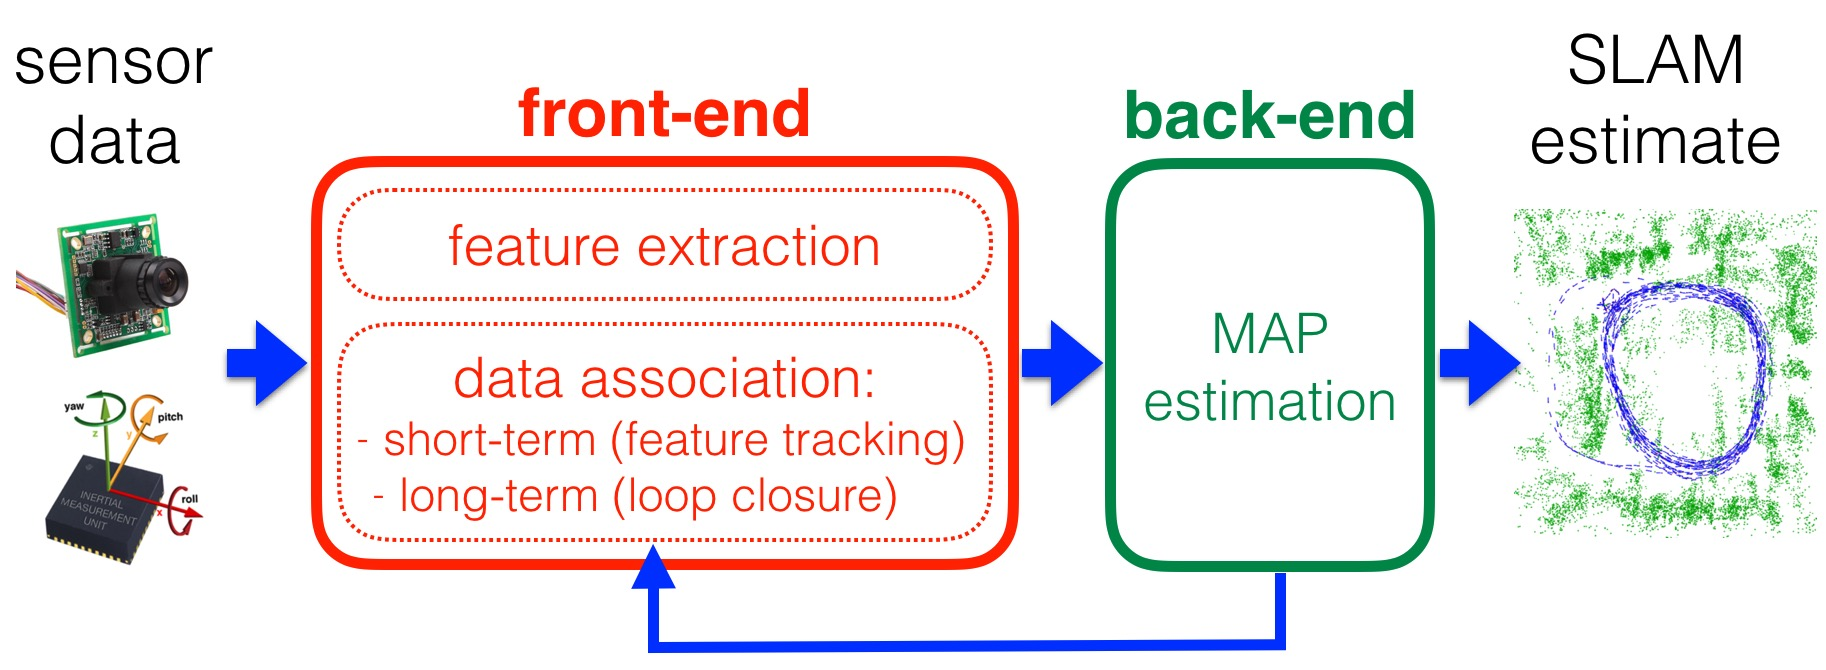
\includegraphics[width=0.7\textwidth]{figures/slamStructure}
    \caption{Front-end and back-end in a typical SLAM system\cite{cadena2016past}}
    \label{fig:slamStructure}
\end{figure}
\\The structure of SLAM system is mainly divided into two parts: front-end and back-end
The front-end extract features from sensor data and associate them to the model used to make predictions, then the back-end does estimation of robot state and the map using this model produced by front-end. As you can see in the figure \ref{fig:slamStructure}, this process forms a continuous process of tracking and update.\\
Classical formulations of SlAM is to take probabilistic approaches such as models based on Maximum Likelihood Estimation, Maximum-a-posteriori (MAP) estimation, EKF(Extended Kalman Filters), and particle filters.\\
Many of the popular SLAM algorithm models it as a maximum-a-posteriori estimation problem  by taking probability approach. And usually using a factor graph to show relationships and constraints between variables. In these models, often an observation or measurement model
is used to represent the probability of observe measurements given the state of robot, given some random measurement noise that usually model to be under a zero-mean Gaussian distribution. By using Bayes theorem, the MAP estimate, in which the posterior is the probability of robot state given a measurement, can be calculated given some prior belief of the robot state. In the case that there is no prior information known about robot state, the MAP estimate would simply become a maximum-likelihood-estimate. When we are given a set of independent robot states and measurements, these variable would become factors(nodes) in the factor graph, and their probabilistic relationships would become the constraints(edges) in the factor graph.\\
Factor graph allows us to visualize our problem in a simple way and provides an insight into how the variables are related together by their constraints. \ref{fig:factorgraph} from the paper have shown an example of it for a simple SLAM problem.
\\
\begin{figure}[h]
    \centering
    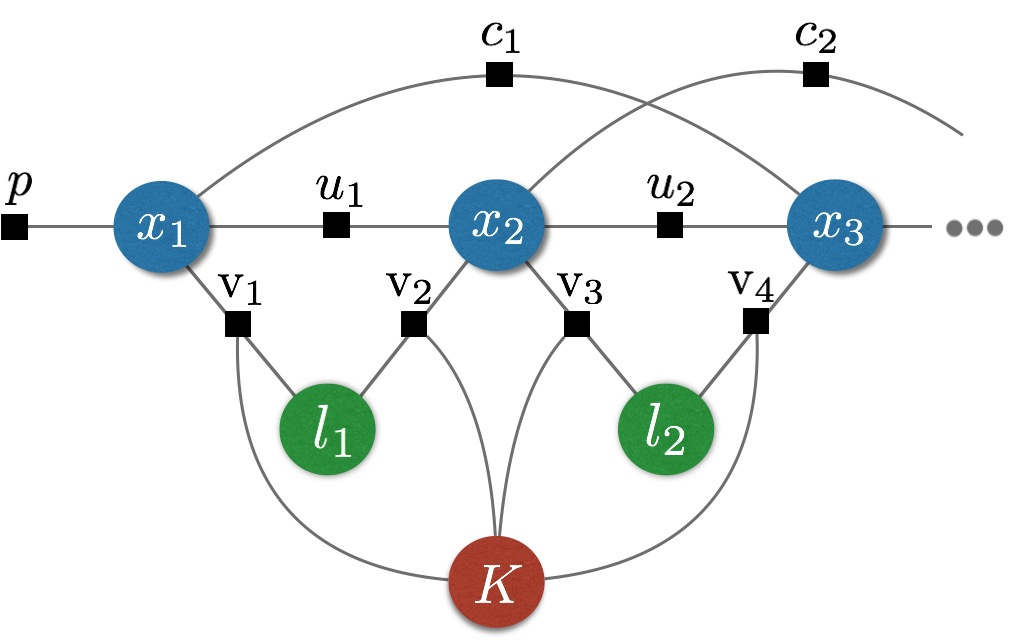
\includegraphics[width=0.7\textwidth]{figures/factorgraph}
    \caption{SLAM as a factor graph\cite{cadena2016past}}
    \label{fig:factorgraph}
\end{figure}
\\
As explained in \cite{cadena2016past}: \lq\lq Blue circles denote robot poses at
consecutive time steps ($x1$, $x2$ ...), green circles denote landmark positions
($l1$, $l2$ ...), red circle denotes the variable associated with the intrinsic
calibration parameters ($K$). Factors are shows are black dots: the label \lq\lq $u$\rq\rq marks factors corresponding to odometry constraints, \lq\lq $v$ \rq\rq marks factors corresponding to camera observations, \lq\lq $c$\rq\rq denotes loop closures, and \lq\lq $p$\rq\rq denotes prior factors."\\
\\
When calculating the MAP estimate of robot state, we can transform the problem into minimizing the negative log of posterior, assuming the noise is zero-mean Gaussian distributed, this becomes a non-linear least squares problem, since we will be minimising the measurement error's $l2$ norm. This method is similar to the BA (Bundle Adjustment) method in computer vision area, which minimise the reprojection error. However factor graph can not only contain visual and geometry factor, but also a variety of data from different sensors. Also the MAP estimate is calculated every time a measurement is arrived, instead of performing calculation  after all the data is given.\\
Different from factor graph optimization, a similar approach is called pose graph optimization, which estimate trajectory of robot using measurements between relative poses as constraints, and optimized these poses to achieve better accuracy trajectory.
\\
Other than optimization-based estimation, some filtering approach using EKF model have also achieve great results, such as MSCKF(Multi-State Constraint Kalman Filter of Mourikis and Roumeliotis)\cite{mourikis2007multi}, EKF is used for performing filtering on the linearised point of estimate, and have shown to be accurate in visual-inertial navigation.
\\
In terms of the representation of the map, one way is to have a group of features or landmarks in 3D, these features are usually extracted from sensor images to be allow easy distinguishable from environment, such as edges and corners. The method used to extracting features from images are well-established within computer vision area, using descriptors like ROB, SIFT, and SURF. The discriminative and repetitive properties of landmarks allow the correspondence of each landmark and sensor measurement(image), and then via triangulating, the robot is able to compute the relative pose between measurements and geometric information about landmarks, therefore achieve localization and mapping.\\
\\
Other than feature based approach, sometimes raw dense representation of the environment is used. different than extracting landmarks, this approach stores a dense 3D map using high resolution points, the 3D geometry of environment is described by these vast amount of points, so called point clouds. With stereo or depth cameras, lase r depth sensors, 3D information of the points can be easily obtained, therefore this method is popular in RGB-D SLAM. Sometimes, these points doesn't only stores simple 3D information, in Elasticfusion\citep{whelan2015elasticfusion}, each 3D point is represented by a surfel, which is a disk with certain radius centred by the 3D point and stored information such as normal vector of that point on the surface and color. These suefel disk combine together can encode the geometry of environment better than simple points.\\
At more a higher level than raw, unstructured points, dense related element that partitioned by space is also used to represent surface and boundaries, such as surface mesh models(connected polygons formed by points) and implicit surface representations like octree and occupancy grid. KinectFusion\citep{newcombe2011kinectfusion} storing surfaces using volumetric representation by uniformly subdivide a 3D physical space into a 3D grid of fixed size voxels, voxels defining surface has a zeros value of the truncated
signed-distance function (TSDF) function that stores distance information relative to the surface. We can see that represent the environment in these types of dense data requires huge amount of storage, however they give very low level geometry information which is suitable for 3D reconstruction and rendering.\\
\\
Comparing feature-based and dense SLAM methods, for the purpose of this project, we will use dense SLAM algorithm such as Elasticfusion\citep{whelan2015elasticfusion} for 3D reconstruction, since it maintains a dense 3D surfel map that make use of all the information about the environment from sensor thus more robust for localization and mapping.\\

\subsubsection{Kinectfusion}
KinectFusion\cite{newcombe2011kinectfusion} is a dense RGB-D SLAM method that enables high quality 3D reconstruction and interaction in real time.
This method make use of mobile low cost RGB-D camera, scanning the environment in real time and acquire 3D point information about the space. During the reconstructing process, holes caused by absence of depth measurement in original 3D point cloud is filled, and model is more refined by repetitive scanning over time.\\
Firstly the 3D points reading are then stored in a 3D vertex map and their normal vectors are calculated by reprojection of neighbouring vertexes. After that the camera pose is tracked by  using Iterative Closest Point (ICP)\citep{chen1992object}\citep{besl1992method} algorithm to align current 3D points with the previous frame. In ICP algorithm, first the corresponding point of each current 3D point is found by doing  projective data association, which reprojects each previous point into image coordinates and use this to look up current vertexes that may be correspondence points. In the second part these correspondences are tested by calculated distance and angle between them and reject any outliers that are beyond certain threshold. Please be noted that the running of ICP in real time is because the use of GPU to parallel processing a current vertex per thread, according to the original paper.\\
\begin{figure}[h]
    \centering
    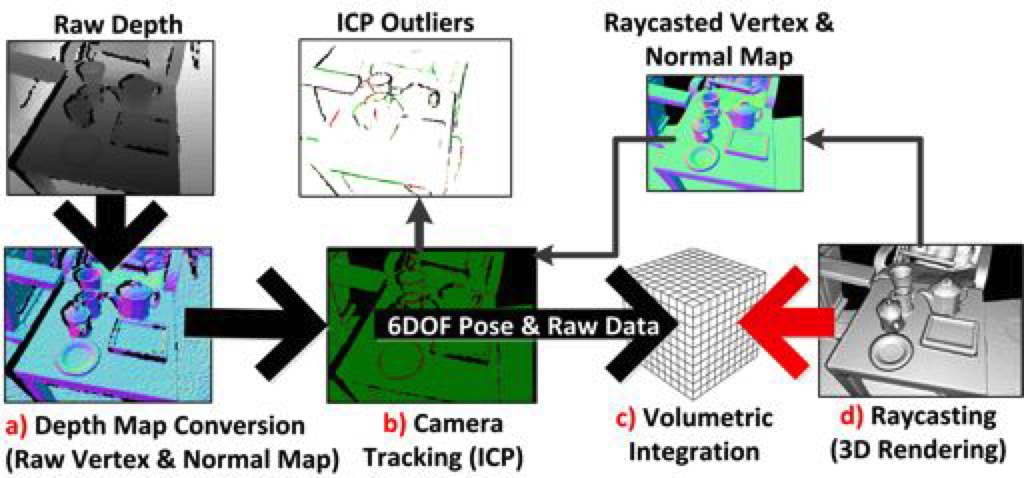
\includegraphics[width=0.7\textwidth]{figures/kinec}
    \caption{Overview of tracking and reconstruction pipeline
from raw depth map to rendered view of 3D scenem\cite{newcombe2011kinectfusion}}
    \label{fig:kinec}
\end{figure}
\\The structure of KinecFusion is given in Fig \ref{fig:kinec} from original paper. The result of ICP is a transformation matrix from previous camera pose to the current pose, which is later used for converting the coordinates of current vertexes into the global coordinate frame. These coordinate data is then fused into the current model that uses a volumetric representation, as mentioned before. The 3D space is uniform divided into fixed size voxel grid. The geometry of surface is implicitly stores in these voxels by having zero values of Truncated Signed Distance Functions (TSDFs) at the surface, positive value in the front of surface, and negative at the back of it. Also, to improve efficiency and minimise storage usage only a truncated area around the surface is actually stored, thus the name "truncated".\\
When integrating the current vertexes into voxel grid, each voxel is perspective projected back onto the image to calculate the difference between it and the measurement depth of this coordinate. The distance difference is then normalized to maximum TSDF distance and updated using weighted average with   previous value. Similar to the implementation of tracking stage, the integration and update process also make use of GPU parallel processing, each thread is assigned a slice of of grid along the $Z-axis$, and sweep through each voxel by its $(x,y)$ position for processing, as shown in Fig \ref{fig:kin}.\\
\begin{figure}[h]
    \centering
    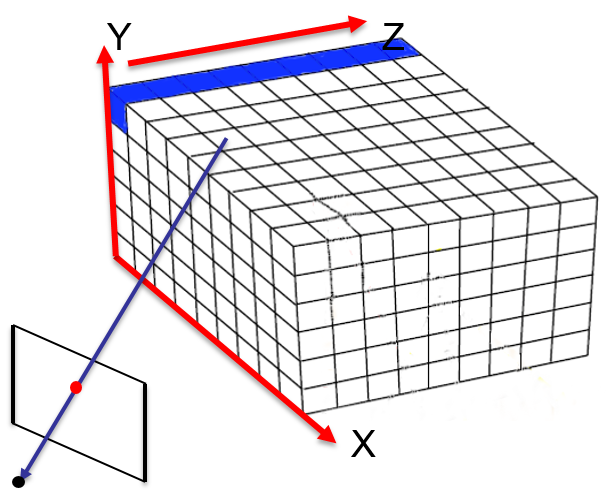
\includegraphics[width=0.5\textwidth]{figures/kin}
    \caption{Volumetric Integration using GPU thread \cite{1_yin_2016}}
    \label{fig:kin}
\end{figure}\\
Finally, in order to render the 3D reconstructed surface raycasting is performed. This is done by having each GPU thread to follow a ray from the camera center along one pixel in the image into the voxel grid in camera coordinate space, the ray is extended until a zero-crossing voxel is met, this voxel represents the surface point observed by this pixel and the position is extracted by doing a trilinear interpolation on this voxel point. And the normal at this position is calculated by find the surface gradent of TSDF values around the position. With these information for each pixel, a live 3D reconstruction view from camera view point can be rendered using camera's pose and intrinsic information.


\subsubsection{Keyframe-Based Visual-Inertial SLAM Using
Nonlinear Optimization}
Other than using depth sensor with RGB camera, another kind of sensor equipped on the Google Tango table is Inertial Measurement Unit (IMU). Okvis\cite{leutenegger2015keyframe} is a sparse feature-based SLAM approach that tightly coupled IMU measurement with stereo visual measurement using nonlinear optimization.\\
Usually in optimization-based visual SLAM, the structure of geometry is to relate camera poses using landmarks, and optimization is performed to minimize the error of landmark reprojection in different observing frames. However, in visual inertial SLAM, the IMU measurement is used to add additional constraint between camera poses and speed and estimation biases from gyroscopes and accelerometers. The structure graph from original paper is shown in Fig \ref{fig:kinec} with detail labelling of different variables and constraints.\\
\begin{figure}[h]
    \centering
    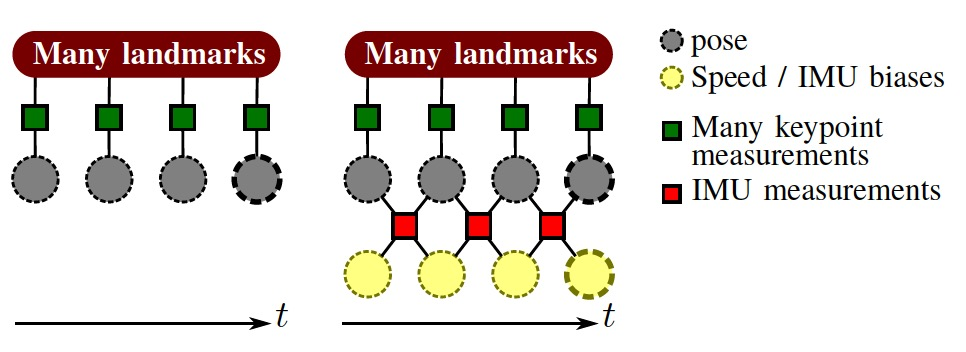
\includegraphics[width=0.7\textwidth]{figures/okvis}
    \caption{graph of variables and their relationships in visual SLAM on the left and visual intertial SLAM on the right \cite{leutenegger2015keyframe}}
    \label{fig:okvis}
\end{figure}\\
In order to tightly couple the visual and inertial measurements, a joint nonlinear cost function that contains both visual reprojection error term and IMU error term is created. These both errors are eliminated by optimizing this one error function.\\
To reduce complexity and ensuring real time operation, a fixed size temporal window of robots poses and relative states is maintained, and old robot poses will be marginalized out as new frames are inserted.\\
In the visual frontend, a sparse map of frames and landmarks is stored. For each new frame, keypoints are extracted using SSE(Streaming SIMD Extensions)-optimized Harris corner detector and BRISK(Binary Robust Invariant Scalable Keypoints) descriptor, their 3D positions are then triangulated by stereo and put into the sparse map. During the process landmarks and keypoints are brute-forcely matched and outliers are rejected by using predicted pose from IMU data. In the optimization window, two kind of frames is maintained, first is a temporal window of the S most recent frames, second is N keyframes in the past. A frame is determined as keyframe if the number of matched points with previous frame is less than 50 to 60\%  of the number of detected keypoints.\\
\begin{figure}[h]
    \centering
    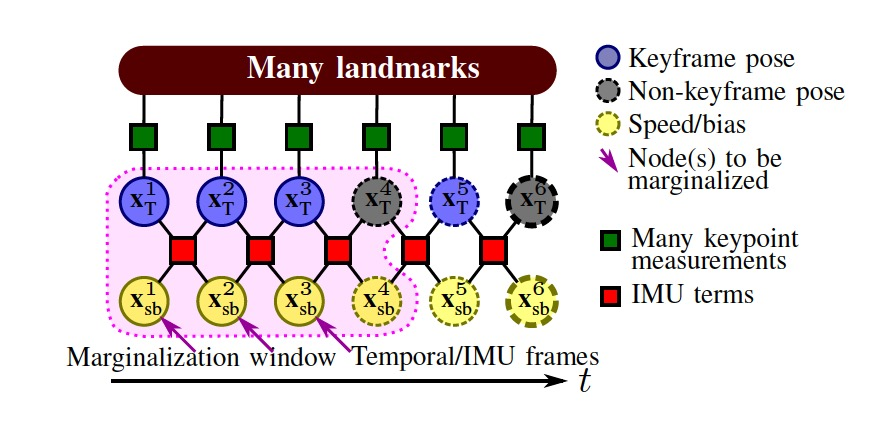
\includegraphics[width=0.7\textwidth]{figures/okvis1}
    \caption{Graph of initial marginalization window \cite{leutenegger2015keyframe}}
    \label{fig:okvis1}
\end{figure}
\begin{figure}[h]
    \centering
    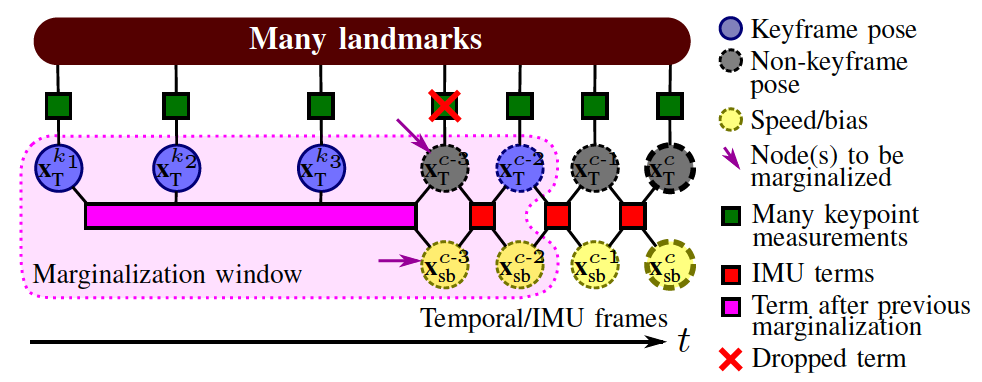
\includegraphics[width=0.7\textwidth]{figures/okvis2}
     \caption{Graph for marginalization in the first case \cite{leutenegger2015keyframe}}
    \label{fig:okvis2}
\end{figure}
\begin{figure}[h]
    \centering
    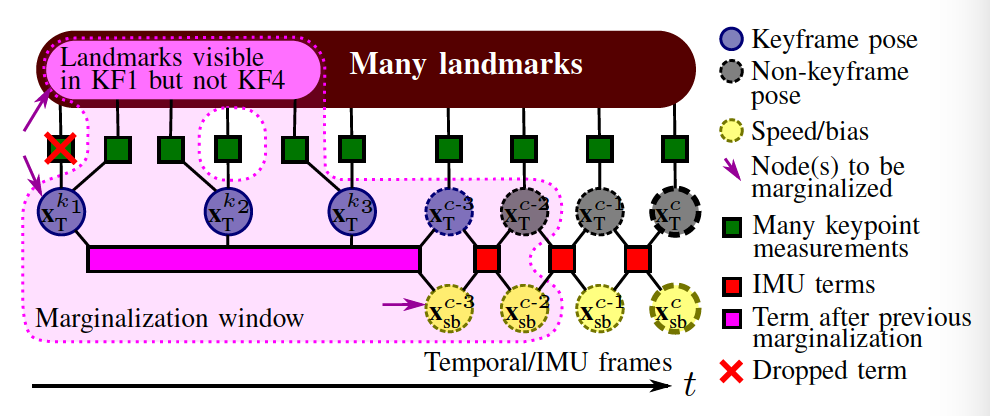
\includegraphics[width=0.7\textwidth]{figures/okvis3}
   \caption{Graph for marginalization in the second case \cite{leutenegger2015keyframe}}
    \label{fig:okvis3}
\end{figure}
In the marginalization process, initially the first $N+1$ frames forms the marginalization window, as shown in Fig \ref{fig:okvis1}. When a new frame is inserted into the marginalization window, there are two ways to marginalize old state. If the oldest frame in temporal window is not a keyframe, then the state of that frame with its measurements, speed and biases will be dropped, as shown in Fig \ref{fig:okvis2}. On the other hand if it is a keyframe, landmarks that are visible in first temporal frame but in most recent keyframe is also dropped, as shown in Fig \ref{fig:okvis3}.\\

\subsubsection{Elasticfusion}
Elasticfusion\cite{whelan2015elasticfusion} is a RGB-D dense SLAM method for 3D reconstruction in room scale without using pose graph , it also use surfels to represent the map instead of voxel grid. In the scanning process, it iteratively check for local and global loop closures and refine the map by using a deformation graph to apply non rigid deformation to the surface. However, while this approach has achieved great results in room scale, it may be difficult to use it on bigger or outdoor scenes.\\
In the surfel map, each surfel stores information about local surface area around the center to reduce holes on the surface, these information includes position, normal, color and radius. The radius is larger as distance between image center and surfel is longer. The surfels are extracted from point cloud using the same method as in \citep{keller2013real}. But differently, in here the surfels are divided into active and inactive parts. Inactive parts are the surfels that have not been observed for a given time period. OpenGL shading language is used to manage the surfel map and update, fusion and render the view. \\
First, in camera pose tracking step, dense frame-to model camera tracking is used, geometric and photometric pose estimations are combined into a joint cost function to be minimised. geometric error is calculated using frame to model projective data association and ICP algorithm as in kinecFusion\citep{newcombe2011kinectfusion}, and photometric error is gain by calculating the intensity difference between current RGB image and backprojected image. Noted that here in the tracking process only active surfels are used.\\
The realignment of map is done by applying non rigid deformation using deformation graph, it is constructed for each frame for efficiency with nodes sampled uniformly from the surfels which is same as in DynamicFusion\citep{newcombe2015dynamicfusion}. Each node have a rotation matrix and position vector that represents optimization parameter and neighbourhood of each node forms the edge of them. Each surfel has a set of influencing nodes that affects the deformation of that surfel.\\
After camera pose tracking for each frame, global loop cloure is checked to recover from drifts and realign the camera pose. The frame information from past is stored in a randomized fern encoding database using same technique as\cite{glocker2015real}, it allows storing and matching frames without putting redundent information into the database. If a high quality matched is found, points are sampled from surfels to build constraints that are used to optimize the deformation graph.\\
If no global loop closure is found then local model to model loop closure is checked by try to register the part of inactive model with active model under the same frame, similar method is used when high quality alignment is found, constraints are extracted and fed into  the deformation graph, then the inactive surfels in this alignment is reactivated to allow for fusion into the map.\\
After the optimization, deformation graph is applied to the surface by using a weighted distance method to calculate the transformation of surfel by its influencing nodes. The new surfel map is then updated and new image under current viewpoint is rendered by OpenGL.\\ 


\subsection{Related Solution}
\subsubsection{CHISEL}
CHISEL\citep{klingensmith2015chisel} is a a system for large scale 3D reconstruction solution in real time on Google Tango. It uses dynamic spatially-hashed truncated signed distance field\citep{niessner2013real} to represent the map and combine visual and odometry data as odometry frontend. To save memory and computation power, space that does not contain surfaces is culled out. By using space carving, even though Tango's depth sensor provides data with high noise, high quality reconstruction is still achieved in large scenes. To generalise the solution onto other mobile devices that does not have a powerful GPU, no parallel processing is used to utilise the general purpose GPU provided on Google Tango tablet.\\
In the pose estimation stage, CHISEL uses the pose estimated provided by Tango platform as a black box, by try to register each depth scan with the model, poses are optimised in the same way as using ICP algorithm, this allows small drifts between frames to be recovered, however during long process of scanning large scene, drifts will still occur due to the lack of global loop closure.\\
Since the map is stored using spatially-hashed data structure, insert and look up is  very fast. The map is divided into chunks, and each chunk is a fixed grid of 
voxels. These chunks are then spatially-hashed into a spatial 3D hash map. When looking for chunks that need to be updated or drawn, a camera frustum is created for culling chunks that do not intersect with the frustum or not have a depth data, the rest of chunks left is then processed for update or drawn.
For fusing depth scan data into the model, projection mapping is used to compare the depth value on image with the projected visual hull of a voxel, the result is then used to update the TSDF value and weight of that voxel.
In the rendering stage, incremental Marching Cubes is used to generate triangle meshes for the chunk when it is been updated by a depth scan, triangles are generated at the zero isosurface of the TSDF volxel grid.\\
CHISEL has shown a nice approach to scanning large scene for high quality 3D reconstruction, however it fails to maintain global consistency of the map by lacking detection of global loop closure. 


\section{Body of report}
The central part of the report usually consists of three of four chapters detailing the technical work undertaken during the project. The structure of these chapters is highly project dependent. They can reflect the chronological development of the project, e.g. design, implementation, experimentation, optimisation, evaluation etc. although this is not always the best approach. However you choose to structure this part of the report, you should make it clear how you arrived at your chosen approach in preference to the other alternatives documented in the background. If you have built a new piece of software you should describe and justify the design of your program at some high level, possibly using an approved graphical formalism such as UML. It should also document any interesting problems with, or features of, your implementation. Integration and testing are also important to discuss in some cases. You need to discuss the content of these sections thoroughly with your supervisor.\\

============\\
The plan of this project is to start with simple sample project on Google Tango Tablet, using the Tango C API, based on exist C++ code for Okvis\cite{leutenegger2015keyframe}, to iteratively build out the solution step by step, so that milestones are available if a certain stage is unable to complete before the project deadline.\\
In this project the goal is run ElasticFusion\citep{whelan2015elasticfusion} on Google Tango Tablet for real time 3D reconstruction, but the algorithm will be adapted to fit into the Tango platform, also to make use of the Tango motion tracking and depth perception API. Given that Tango's camera pose estimation already make use of RGB-D and IMU sensor data, the pose tracking could possibly be replaced with 3D pose gain directly from Tango. Also, camera frame and 3D point cloud data for a time point can be acquired with the API. However, although the Tango 3D Reconstruction Library C provides functions and structs reconstruct 3D suface using mesh or voxel grid, it is different than the surfel map that we will be using for ElasticFusion\citep{whelan2015elasticfusion}. However, it will be worth to study the sample project of building mesh and rendering on screen.\\
First, we need to set up a simple demo Google Tango Android application for motion tacking that output real time pose data into the logs.\\
Then camera frames needed to be rendered on screen in real time with buttons to resume and pause the rendering.\\
Next step is to make use of the mesh builder in Tango 3D Reconstruction Library for fusing point clouds and use OpenGL to render it on screen from the camera view point.\\
After that we can build out the structs and functions for surfel map and global map representation used in ElasticFusion\cite{whelan2015elasticfusion}, in which the surfels are divided into active and inactive types according the time it is last observed.\\
With the surfel map classes, integration with Tango could be done by try to extract surfels from point cloud data and then render the surfels into the screen.\\
Then the structs and functions for deformation graph, its nodes and surface constraints will be built to allow for non rigid deformation of the surface.\\
In order to perform the optimization using surface constraints, global and local loop closure needs to be done. For global loop closure, ElasticFusion\cite{whelan2015elasticfusion} uses randomised fern encoding database to store frame information and check for match frames. Therefore fern and frame structs and this store, lookup mechanism needs to be implemented.\\
With global loop closure in place, this can be tested out by manually triggering the loop closing and see whether deformation graph is applied, which will cause the surfaces to be realigned, and camera pose be updated.\\
If this is successful, local loop closure can also be done using model-to-model tracking by trying to register the active and inactive point clouds together under the current frame view point. This is done by using the same tracking and optimization process in global loop sure.\\
It will be the ideal case if the above is all achieved before the project deadline, since this is a very challenging project. And if at a certain stage it is realised that it could not be done before the deadline, the progress can be fall back to the previous milestone and start clean up and report write up.\\ 
However, extension and optimization could be done if more time is given and basic solution is completed. Until here the 3D reconstruction process will be running on Tango tablet's NVIDIA Tegra K1 processor without utilizing the CUDA feature on it to improve performance by parallel processing. A optimization could be to use CUDA in the camera tracking process. Also on the application side, extra features can be added such as saving the reconstructed surfel map on the Tango tablet, add an interactive view of reconstructed 3D surface map on the screen to allow for drag and zoom operation, showing the camera's current pose on the map. Further more, demo application and be built to utilising the augmented reality ability on Tango platform, such as placing a virtual static object on the 3D reconstructing surface.\\
The project timeline is shown in Fig \ref{fig:tiemline2} with each task corresponding to a stage above.


\newpage

\begin{figure}
\centering
    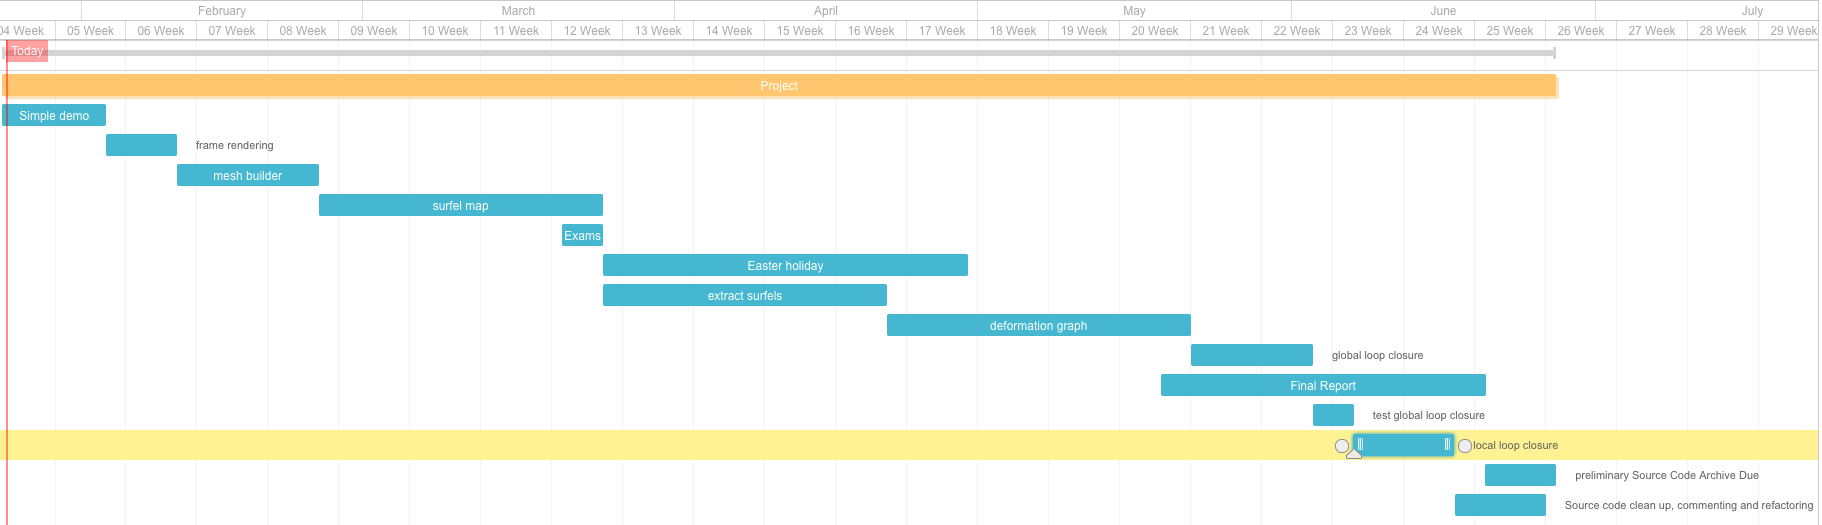
\includegraphics[angle=90,width=\textwidth,height=\textheight,keepaspectratio]{figures/timeline2}
   \caption{Graph for project timeline}
    \label{fig:tiemline2}
\end{figure}

\newpage

\section{Evaluation}


Be warned that many projects fall down through poor evaluation. Simply building a system and documenting its design and functionality is not enough to gain top marks. It is extremely important that you evaluate what you have done both in absolute terms and in comparison with existing techniques, software, hardware etc. This might involve quantitative evaluation, for example based on numerical results, performance etc. or something more qualitative such as expressibility, functionality, ease-of-use etc. At some point you should also evaluate the strengths and weaknesses of what you have done. Avoid statements like "The project has been a complete success and we have solved all the problems asssociated with blah...; - you will be shot down immediately! It is important to understand that there is no such thing as a perfect project. Even the very best pieces of work have their limitations and you are expected to provide a proper critical appraisal of what you have done.\\

=============\\


The evaluation of this project is intended to use the same mechanism as in original ElasticFusion\citep{whelan2015elasticfusion} paper, as the goal of this project is to deploying this algorithm on Google Tango tablet.\\
In order to measure the performance of this solution by quantity and quality. Both algorithm and computational performance need to be benchmarked.\\
Both 
A. Trajectory Estimation
To evaluate the trajectory estimation performance of our approach
we test our system on the RGB-D benchmark of Sturm
et al. [22]. This benchmark provides synchronised ground truth
poses for an RGB-D sensor moved through a scene, captured
with a highly precise motion capture system.  We use the absolute
trajectory (ATE) root-mean-square error metric (RMSE) in
our comparison, which measures the root-mean-square of the
Euclidean distances between all estimated camera poses and
the ground truth poses associated by timestamp [22].
 
 
B. Surface Estimation
We evaluate the surface reconstruction results of our approach
on the 
 This
benchmark provides ground truth poses for a camera moved
through a synthetic environment as well as a ground truth 3D
model which can be used to evaluate surface reconstruction
accuracy. 

Computational Performance


​The evaluation of this project is intended to use the same mechanism as in original ElasticFusion\citep{whelan2015elasticfusion} paper, as the goal of this project is to deploying this algorithm on Google Tango tablet.\\
In order to measure the performance of this solution by quantity and quality. Both algorithm and computational performance need to be benchmarked.\\
For the algorithm, trajectory accuracy can be tested using sample data sets to provide RGB-D input, then the trajectory output can be compared with the ground truth data that is obtained by using industrial standard system. The root mean square distance between every estimated pose and ground truth pose can be calculated to provide error at each timepoint. In the 3D reconstruction part, similar method can be used to compare the reconstructed surface to benchmark data for accuracy estimation. However, since the post data and image input are provided by Tango platform, a way is needed to fed the benchmark data into Tango.\\
For computational Performance, we can simply plot the frame rate during the process of 3D scanning to check if it is within the acceptable range for real time SLAM algorithm.\\
​The evaluation of this project is intended to use the same mechanism as in original ElasticFusion\citep{whelan2015elasticfusion} paper, as the goal of this project is to deploying this algorithm on Google Tango tablet.\\
In order to measure the performance of this solution by quantity and quality. Both algorithm and computational performance need to be benchmarked.\\
For the algorithm, trajectory accuracy can be tested using sample data sets to provide RGB-D input, then the trajectory output can be compared with the ground truth data that is obtained by using industrial standard system. The root mean square distance between every estimated pose and ground truth pose can be calculated to provide error at each timepoint. In the 3D reconstruction part, similar method can be used to compare the reconstructed surface to benchmark data for accuracy estimation. However, since the post data and image input are provided by Tango platform, a way is needed to fed the benchmark data into Tango.\\
For computational Performance, we can simply plot the frame rate during the process of 3D scanning to check if it is within the acceptable range for real time SLAM algorithm.


\section{Conclusions and Future Work}
The project's conclusions should list the things which have been learnt as a result of the work you have done. For example, "The use of overloading in C++ provides a very elegant mechanism for transparent parallelisation of sequential programs", or "The overheads of linear-time n-body algorithms makes them computationally less efficient than O(n log n) algorithms for systems with less than 100000 particles". Avoid tedious personal reflections like "I learned a lot about C++ programming...", or "Simulating colliding galaxies can be real fun...". It is common to finish the report by listing ways in which the project can be taken further. This might, for example, be a plan for doing the project better if you had a chance to do it again, turning the project deliverables into a more polished end product, or extending the project into a programme for an MPhil or PhD.\\


\section{Bibliography}
This consists of a list of all the books, articles, manuals etc. used in the project and referred to in the report. You should provide enough information to allow the reader to find the source. In particular references must contain all the information regarding the publication of the paper and must be consistently formatted. Usually this means:\\
* For journals: Authors, Title, Journal, volume number, issue number, page number, publisher, month, year.
* For conferences: Authors, Title, Conference name, Place where held, publisher, page number, month, year.
* For technical reports: Authors, Title, institution, Technical report number, month, year.
* For web references: Authors, Title, Web-reference, date accessed.
* URLs are optional for published work but preferred.\\
A weakness of many reports is inadequate citation of a source of information. It's easy to get this right so there are no excuses. Each entry in the bibliography should list the author(s) and title of the piece of work and should give full details of where it can be found. For example:\\
1 Bennett, A.J., Field, A.J. and Harrison, P.G., "Modelling and Validation of Shared Memory Coherency Protocols", Performance Evaluation, 1996, Vol. 27  28, 1996, pp. 541-562. rather than just listing the source as "Performance Evaluation 1996".
Using a reference management programme can make your life simpler.See for example Bibdesk,JabRef,RefWorks, etc.\\

\section{Appendix}
The appendices contain information which is peripheral to the main body of the report. Information typically included are things like parts of the code, tables, proofs, test cases or any other material which would break up the theme of the text if it appeared in situ. You should try to bind all your material in a single volume if possible.\\
\section{User Guide}
For projects which result in a new piece of software you should provide a proper user guide providing easily understood instructions on how to use it. A particularly useful approach is to treat the user guide as a walk-through of a typical session, or set of sessions, which collectively display all the features of your system. Technical details of how the package works should be in the body of the report. Keep it concise and simple. The extensive use of diagrams illustrating the package in action prove particularly helpful. The user guide is sometimes included as a chapter in the main body of the report, but is often better in an appendix.\\
\section{Program Listings}
Complete program listings should NOT be part of the report except in specific cases at the request of your supervisor. The project report(s) must be bound in a departmental folder and must include a standard title page produced by the project co-ordinator. More of this nearer the date.\\
You are strongly advised to spend some time looking at the reports of previous project students to get a feel for what's good and bad. In June 1999 we introduced a "Distinguished Project" classification, which is a formal recognition of outstanding projects for which no official prize was awarded. The complete list of prize winners and the other distinguished projects, along with links to the final reports, can be found here.\\
\section{Word Count}
There is no word count for the report as such, but ideally you should not exceed the limit of 40,000 words. Generally, our best projects tend to have the word count in the range of 20,000 - 35,000 words with a few going beyond that. This does not include the Appendices.\\



\bibliographystyle{unsrt}
\bibliography{mybi}

\end{document}
%%% Local Variables: 
%%% mode: latex
%%% TeX-master: t
%%% End: 
